\section{Theoretical Analysis}
\label{sec:analysis}

\subsection{Operating Point}
Firstly, we started by altering the octave script given by the professor to suit the simulation we had made. We then proceeded to get the operating point analysis in order to compare it to the operating point analysis made in the simulation section.\par
Below are two table with the OP for both the gain and output stages:

\begin{center}
  \begin{tabular}{ | c | c | }
    \hline    
    {\bf Name} & {\bf Value [V or A]} \\ \hline
    \input{../mat/OP1}
    \hline
  \end{tabular}
  \captionof{figure}{Theoretical Operating Point Gain Stage}
\end{center}

\begin{center}
  \begin{tabular}{ | c | c | }
    \hline    
    {\bf Name} & {\bf Value [V or A]} \\ \hline
    \input{../mat/OP2}
    \hline
  \end{tabular}
  \captionof{figure}{Theoretical Operating Point Output Stage}
\end{center}

\subsection{Simulating the gain stage}
After doing the OP analysis, we proceeded to simulate the gain stage, that will increase de signal's gain, and the output stage, that will have to regulate the output (due to the high impedance signal from the gain stage).\par
From the gain stage, we have the following gain (dB) plot:\par

\begin{figure}[H] \centering
\includegraphics[width=0.7\linewidth]{../mat/vgain1.pdf}
\caption{Voltage Gain (Gain stage).}
\label{fig:vgain}
\end{figure}


\subsection{Output stage}
For this stage, we also have a voltage gain plot that is in the image below.\par
The plot shows us the gain in dB.

\begin{figure}[H] \centering
\includegraphics[width=0.7\linewidth]{../mat/vgain2.pdf}
\caption{Voltage Gain (Output stage).}
\label{fig:vgain2}
\end{figure}

\subsection{Frequency Response}
Taking into account the all circuit, we can obtain the frequency response (db):\par

\begin{figure}[H] \centering
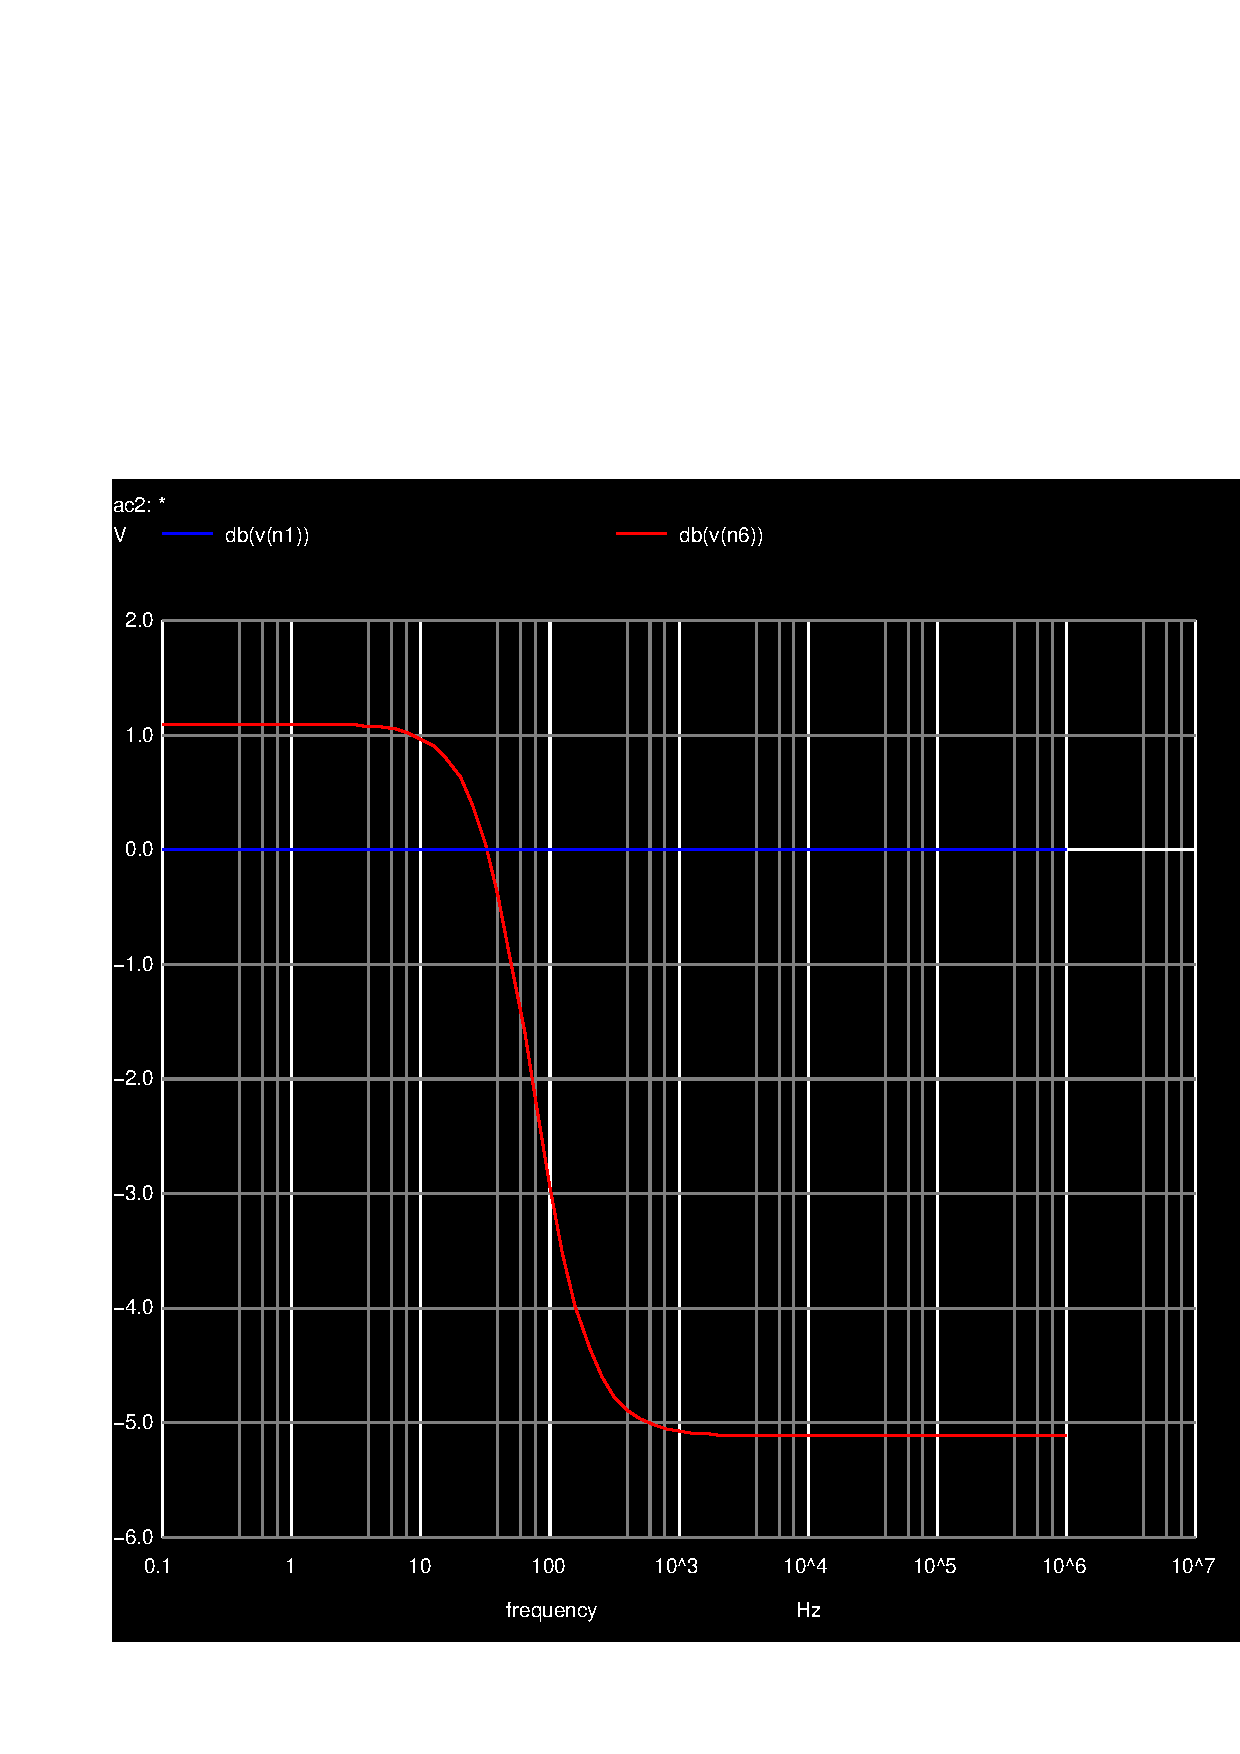
\includegraphics[width=0.7\linewidth]{../mat/fresponse.pdf}
\caption{Frequency Response.}
\label{fig:fresponse}
\end{figure}

\subsection{Impedance}

Summing up, we have these results for impedance:\par

\begin{center}
  \begin{tabular}{ | c | c | }
    \hline    
    {\bf Name} & {\bf Value [$\Omega$]} \\ \hline
    \input{../mat/docImp}
    \hline
  \end{tabular}
  \captionof{figure}{Theoretical Input and Output Impedances}
\end{center}

Ideally, the input impedance ($Z_I$) should be infinite. However, since it is much greater than $R_s$ (source output resistance, which is 100 $\Omega$), our input signal will not be degraded (by the input impedance). Basically, there is no problem to connect this input source through the coupling capacitor and amplifier input.\par
The output impedance of the gain stage is almost 3 times lower than the input inpedance of the output stage, which is not ideal, but this is acceptable, so this two modules can be connected, with some degradation of the signal.\par
